\documentclass{article}
\usepackage{amsmath}
\usepackage{graphicx}
\usepackage{tikz}
\usepackage{pgfplots}
\pgfplotsset{compat=1.18}
\usepackage{sectsty}
\usepackage{float}
\usepackage[left=1in, right=1in, top=1.25in, bottom=1.25in]{geometry}

\sectionfont{\centering}

\title{CalcStudio Math Documentation}
\author{Aayush Koora}

\begin{document}

\maketitle

\newpage
\section{Derivative: Tangent Line at Point}

\noindent
A derivative is the instantaneous rate of change of a function. It answers how fast a function is changing at a specific point \( x = a \).

\vspace{1em}

This is the formal definition of a limit:

\vspace{1em}

\begin{equation}
f'(a) = \lim_{h \to 0} \frac{f(a + h) - f(a)}{h}
\end{equation}

\vspace{1.5em}

\begin{center}
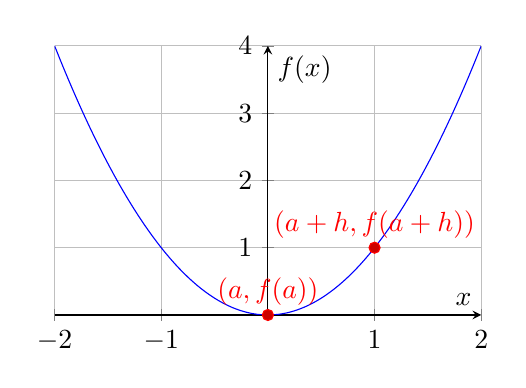
\begin{tikzpicture}
\begin{axis}[
    axis lines=center,
    xlabel=$x$,
    ylabel={$f(x)$},
    grid=both,
    width=7cm,
    height=5cm,
]
\addplot [
    domain=-2:2,
    samples=100,
    color=blue,
]
{x^2};
\addplot+[
    only marks,
    mark=*,
    nodes near coords,
    point meta=explicit symbolic,
] coordinates {
    (0, 0)[$(a, f(a))$]
    (1, 1)[$(a+h, f(a+h))$]
};
\end{axis}
\end{tikzpicture}
\end{center}

\vspace{1.5em}

\noindent
We can decrease \( h \) until it is infinitely small. As the distance between the two points (\( h \)) approaches 0, we get the instantaneous slope of \( f(x) \) at point \( a \).

\vspace{1em}

\noindent
A tangent line is a line that touches a function at one point and has the same slope as that instantaneous point.

\vspace{1em}

\noindent
We can model a tangent line like this:

\vspace{1em}

\begin{equation}
y = f(a) + f'(a)(x - a)
\end{equation}

\vspace{1em}

\begin{center}
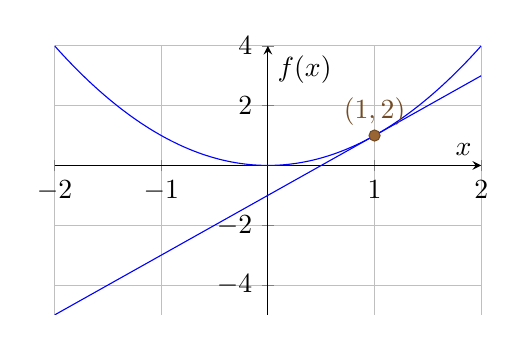
\begin{tikzpicture}
\begin{axis}[
    axis lines=center,
    xlabel=$x$,
    ylabel={$f(x)$},
    grid=both,
    width=7cm,
    height=5cm,
]
\addplot [
    domain=-2:2,
    samples=100,
    color=blue,
]
{x^2};
\addplot [
    domain=-2:2,
    samples=100,
    color=blue,
]
{2*x-1};
\addplot+[
    only marks,
    mark=*,
    nodes near coords,
    point meta=explicit symbolic,
] coordinates {
    (1, 1)[$(1, 2)$]
};
\end{axis}
\end{tikzpicture}
\end{center}

\newpage

\section{Integral: Area Under a Curve/Riemann Sums}

\noindent
An integral is the area under a curve. We can approximate the area under a curve using riemann sums.

\vspace{1em}

\begin{figure}[H]
    \centering
    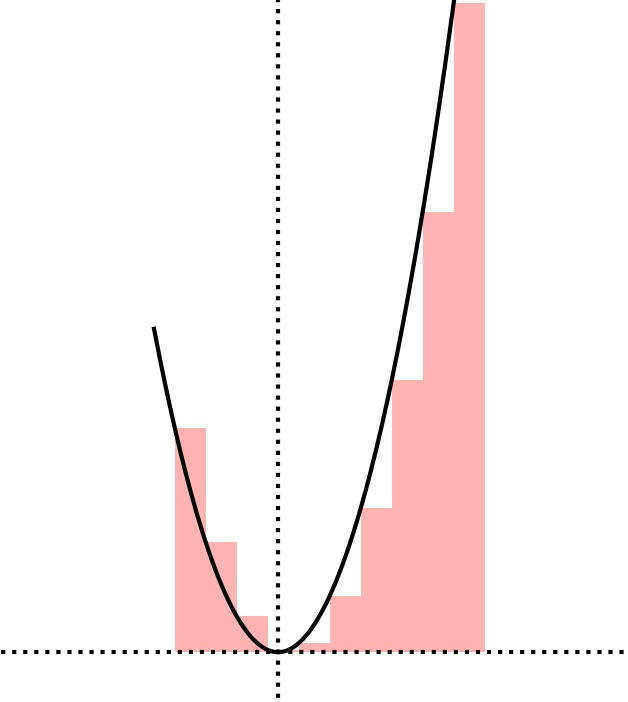
\includegraphics[width=0.4\textwidth]{integral1.jpeg}
\end{figure}

\vspace{1em}

\noindent
As we use increasingly smaller rectangles, we can get closer to the actual value of the are under the curve.

\vspace{1em}

\begin{figure}[H]
    \centering
    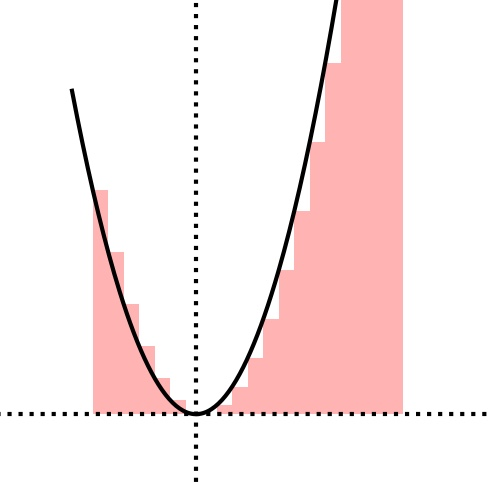
\includegraphics[width=0.4\textwidth]{integral2.jpeg}
    \label{fig:myplot}
\end{figure}

\vspace{1em}

\noindent
We can use a limit statement to find the area under curve using an infinite amount of rectangles. 

\noindent
\vspace{1em}

\noindent
This is the formal definition of an integral:
\begin{equation}
Area = \lim_{n \to \infty} \sum_{i=1}^{n} f(x_i^*) \Delta x
\end{equation}


\vspace{1em}

\noindent
This definition can be rewritten in this notation:

\begin{equation}
Area = \int_a^b f(x)\, dx 
\end{equation}

\vspace{1em}

\begin{figure}[H]
    \centering
    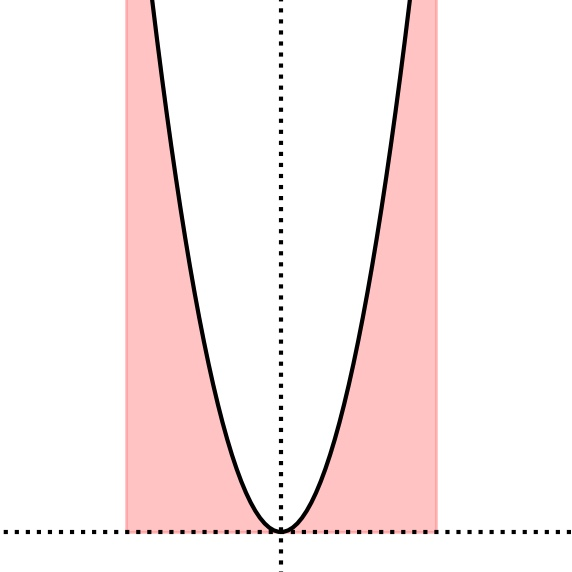
\includegraphics[width=0.4\textwidth]{integral3.jpeg}
    \label{fig:myplot}
\end{figure}

\vspace{1em}

\noindent
The integral finds the exact area under the curve.

\newpage

\section{Multivariable: Gradient Descent}
\noindent
Gradient descent is an interactive algorithm used to minimize the function by following the steepest descent. This algorithm is used in machine learning and can work with multiple parameters.

\vspace{1em}

\noindent
We can model this algorithm using the function \( x^2 = y \)

\vspace{1em}

\noindent
Let's start with a random x value: 5. The first step is to take the derivative of the function at x=5. This value is 10.
\[
f'(x) = 2x \implies f'(5) = 10
\]

\vspace{1em}

\noindent
The next step is to calculate the step size of the next value. By multiplying the learning rate times the derivative of the value.
\[
\Delta x = \eta \times f'(x)
\]

For example, if \( \eta = 0.1 \), then \( \Delta x = 0.1 \times 10 = 1 \).

\vspace{1em}

\noindent
The learning rate \( \eta \) determines how much of a step each iteration of the algorithm takes.

\vspace{1em}

\noindent
The last step is to update the current value by subtracting the step size:
\[
x_{\text{new}} = x_{\text{old}} - \Delta x
\]

Using our example:
\[
x_{\text{new}} = 5 - 1 = 4
\]


\vspace{1em}

\noindent
Now we repeat this process: calculate the derivative at the new \( x \), multiply by the learning rate, update \( x \), and so on, until the step size \( \Delta x \) is smaller than a threshold (e.g., 0.001) or a maximum number of iterations is reached.

\vspace{1em}
\noindent
This iterative procedure allows the algorithm to converge to the function's minimum.

\end{document}
